\chapter{Revisão Bibliográfica}

Nesse capítulo será apresentada uma revisão bibliográfica dos tópicos concernentes a acústica interna de dutos circulares. Os tópicos estão separados em modelos analíticos exatos, modelos analíticos aproximados, trabalhos experimentais, modelos numéricos e trabalhos relacionados ao desenvolvimento e aplicação do método de \textit{lattice} Boltzmann para problemas de acústica.

\section{Modelos Analíticos Exatos} 

A propagação de modos normais (ondas planas) é um problema clássico em acústica e continua tendo importância significativa mediante ao advento de novas tecnologias relacionadas a sistemas de exaustão e sucção. Em geral, pode-se utilizar dois parâmetros para caracterizar o fenômeno da acústica interna de dutos:

\begin{itemize}
    \item a magnitude do coeficiente de reflexão $\|R\|$, razão entre as componentes refletida e incidente da onda no duto, a qual é dada por
    \begin{equation}
        R_{r}\simbolo{$R_{r}$}{Coeficiente de reflexão na terminação do duto} =\frac{Z_{r} - Z_{0}}{Z_{r} + Z_{0}},
        \label{eq:R}
    \end{equation}
    sendo $Z_{r}$\simbolo{$Z_{r}$}{Impedância de radiação} a impedância de radiação e $Z_{0}$\simbolo{$Z_{0}$}{Impedância característica do meio} a impedância característica do meio, definida por $Z_{0} = \rho_{0}c_{0}$, tal que $\rho_{0}$ e $c_{0}$ são, respectivamente, as constantes de densidade média do meio\simbolo{$\rho_{0}$}{Densidade média do meio} e velocidade do som\simbolo{$c_{0}$}{Velocidade do som};
    
    \item coeficiente de correção da terminação normalizado pelo raio do duto $l/a$ em que $a$ é o raio do duto. Tal parâmetro representa o comprimento acústico efetivo do duto. Em outras palavras, o fator $l$ é a quantidade adicional medida a partir da abertura do duto a qual deve propagar a onda incidente antes de ser refletida para o interior do duto com fase invertida. Tal coeficiente de correção da terminação $l$ é dado por
    \begin{equation}
        l = \frac{1}{k} \arctan\!\left(\frac{Z_{r}}{Z_{0} \, \mathrm{i}\simbolo{$i$}{Unidade imaginária}}\right)
        \label{eq:l}
    \end{equation}
    sendo $k$\simbolo{$k$}{Número de onda} o número de onda.
\end{itemize}

Em relação aos parâmetros discutidos acima, a solução exata para o problema de um duto não flangeado na ausência de escoamento foi proposta por \citeonline{levine1948radiation}, porém em boa parte das aplicações práticas dutos transportam escoamentos médios. Para tais circunstâncias, \citeonline{munt1990acoustic} propôs um modelo analítico exato, também baseado na técnica de Wiener-Hopf, em que se considera a presença de um escoamento subsônico no interior do duto. Considera-se nesse modelo as premissas de que o escoamento é uniforme, invíscido e que a camada cisalhante do jato é infinitamente fina. Além disso, o modelo considera a condição de Kutta na borda do duto para lidar com a singularidade da velocidade de partícula nesta região. As Figuras \ref{fig:comp1} e \ref{fig:comp2} apresentam as comparações entre casos com e sem escoamento para um duto não flangeado em termos de $\|R\|$ e $l/a$.

\begin{figure}[ht!]
\centering
  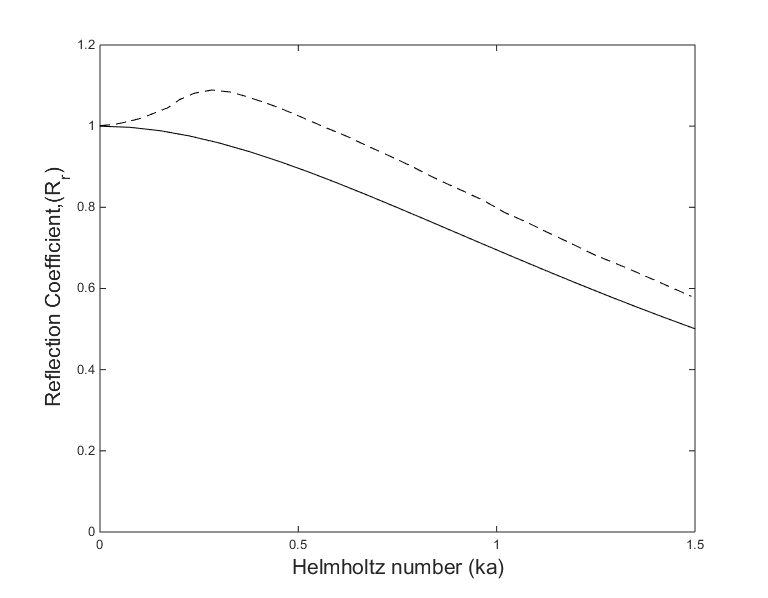
\includegraphics[width=.9\linewidth]{figuras/abs_r_comparacao.png}
  \caption[Magnitudes do coeficiente de reflexão $|R|$]{Resultados analíticos exatos para magnitude do coeficiente de reflexão $\|R\|$ ao final de um duto não flangeado. A linha contínua apresenta o resultado sem escoamento de \citeonline{levine1948radiation} e a linha tracejada apresenta o resultado com escoamento de Mach = 0,15 de \citeonline{munt1990acoustic}.}
  \label{fig:comp1}
\end{figure}

Como é mostrado na Figura \ref{fig:comp1}, a magnitude do coeficiente de reflexão $\|R\|$ aumenta consideravelmente na presença de um escoamento subsônico. Além disso, pode-se perceber que, em algumas frequências, $\|R\|$ torna-se maior do que a unidade, implicando que a amplitude da onda refletida torna-se maior do que a da onda incidente. Este fenômeno ocorre, sobretudo, pela interação do escoamento com a borda do duto, a qual transforma energia cinética rotacional em energia acústica, como discutido por \citeonline{peters1993}. Além disso vale ressaltar que o maior valor de $\|R\|$ está associado com a frequência de desprendimento de vórtices na saída do duto, ou seja, a um número de Strouhal relativo a maximização do desprendimento de vórtices na terminação do duto.  

\begin{figure}[ht!]
\centering
  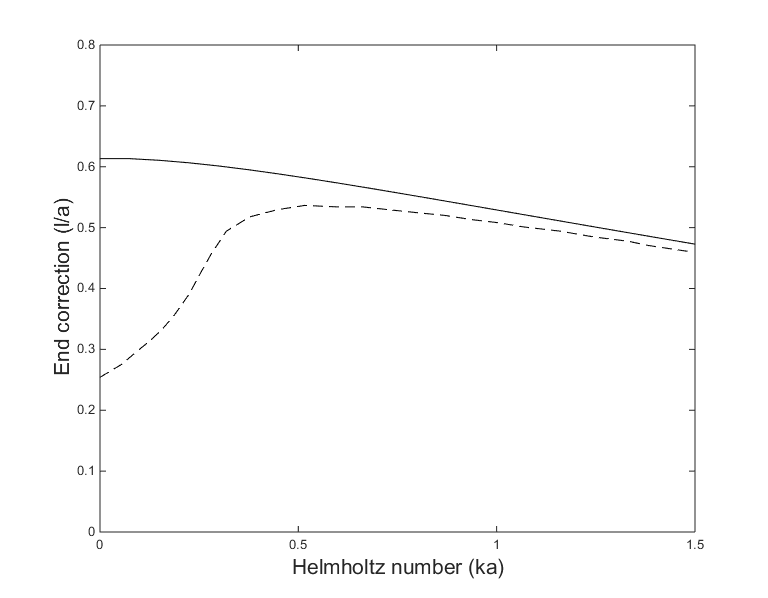
\includegraphics[width=.9\linewidth]{figuras/loa_comparacao.png}
  \caption[Coeficientes de correção de terminação $l/a$]{Resultados analíticos exatos para o coeficiente de correção da terminação normalizado pelo raio $l/a$ de um duto não flangeado. A linha contínua apresenta o resultado sem escoamento de \citeonline{levine1948radiation} e a linha tracejada apresenta o resultado com escoamento de Mach = 0,15 de \citeonline{munt1990acoustic}.}
  \label{fig:comp2}
\end{figure}

De acordo com a Figura \ref{fig:comp2}, a correção normalizada da terminação $l/a$ torna-se consideravelmente menor do que aquela obtida na ausência de escoamento, sobretudo para baixos números de Helmholtz ($ka$)\simbolo{$ka$}{Número de Helmholtz}. Em outras palavras, para baixas frequências e na presença de um escoamento a onda acústica é refletida em uma região mais próxima da abertura, em comparação à situação sem escoamento.

\section{Modelos Analíticos Aproximados}

No que diz respeito a modelos analíticos aproximados, o trabalho de \citeonline{carrier1955sound} foi um dos primeiros a abordar o cálculo do coeficiente de reflexão e correção da terminação com escoamento de exaustão num duto não flangeado. Para tal foi considerado um gás perfeito invíscido com o tipo de escoamento uniforme (\textit{plug}). Nessa abordagem usou-se a mesma metodologia que \citeonline{levine1948radiation} porém acoplando à formulação matemática o método de Prandtl-Glauert.

\citeonline{mani1973refraction} deu prosseguimento a mesma abordagem de \citeonline{carrier1955sound} com escoamento de exaustão, porém considerando a continuidade do deslocamento das partículas acústicas transversais. Esse tipo de solução mostra diversos fenômenos antes não previstos com os outros modelos citados como efeitos de convecção, zonas de silêncio relativo e refrações.

Também na mesma linha de desenvolvimento de \citeonline{carrier1955sound}, \citeonline{savkar1975radiation} desenvolveu um modelo de modos de alta ordem com escoamento de exaustão e sucção do tipo \textit{plug} com variação de temperatura. A continuidade do deslocamento das partículas acústicas transversais também foi considerada, possibilitando assim análises de fenômenos de convectivos.

\citeonline{rienstra1980} também desenvolveu um modelo matemático aproximado para o cálculo dos coeficientes de reflexão e terminação do duto não flangeado. A contribuição desse trabalho foi a inclusão dos parâmetros do meio externo ao duto como velocidade do som, densidade e velocidade de escoamento. Com esse modelo foi possível investigar como o meio externo influencia na acústica interna do duto e as limitações da condição de Kutta.

\section{Trabalhos Experimentais}

Em relação a trabalhos experimentais, \citeonline{ingard1975} investigaram o coeficiente de reflexão em dutos quadrados em regime de escoamento succionado de Mach 0,4. O método de medição se baseou na técnica de dois microfones e os mesmos foram ajustados para números de Helmholtz ($ka$) menores que 0,5. Em vista desse contexto experimental, o autor desenvolveu uma fórmula analítica para o cálculo do coeficiente de reflexão.

Na mesma linha de investigação, \citeonline{davies1987} investigou o coeficiente de reflexão porém com dutos circulares não flangeados e flangeados. O autor destaca que a disposição geométrica da terminação do duto, quando submetida a fenômenos de escoamentos succionados, desenvolve a chamada \textit{vena} contracta, que pode ser estimada e associada com o fator de perda $Kp$\simbolo{$Kp$}{Fator de perda}. Em vista dos procedimentos desse trabalho, o autor compara os resultados com o estudo de \citeonline{ingard1975} e sugere um aperfeiçoamento na equação analítica do cálculo do coeficiente de reflexão.

No que diz respeito a escoamentos de exaustão o trabalho de \citeonline{allam2006investigation} abordou um sistema super determinado de medição para investigação da acústica interna de um duto não flangeado. Para contornar a dificuldade de medição do coeficiente de correção da terminação do duto, surgiu-se como motivação o desenvolvimento de um sistema em que há mais microfones do que incógnitas a serem calculadas, em outras palavras, extendeu-se a metodologia de medição de 2 microfones para mais que 4 microfones. Há de se considerar também que a parte imaginária do número de onda, parte associada com a dissipação de energia por viscosidade, não pode ser obtida quando há escoamento e por isso foi incluída como incógnita. Em linhas gerais esse trabalho permitiu a validação experimental do trabalho de \citeonline{munt1990acoustic} e a consolidação de um sistema confiável de medição para esse tipo de problema.

\citeonline{english2010} investigou também de forma experimental os coeficientes de reflexão e de terminação de dutos circulares com diferentes espessuras. Focando para números de Mach entre 0 e 0,3, seus resultados mostram que os coeficientes de reflexão estão com valores acima dos que são encontrados no trabalho de \citeonline{munt1990acoustic}. O autor explica esse fato relatando que a condição de Kutta subestima o surgimento de vórtices na saída do duto.

\section{Modelos Numéricos}

Já em relação a trabalhos envolvendo métodos numéricos, \citeonline{selamet2001wave} analisaram os coeficientes de reflexão e de terminação de dutos circulares com diferentes terminações sem escoamento. Para isso utilizaram método dos elementos de contorno e concluíram que, dentro dos casos analisados no estudo, dutos com terminações anulares possuem maiores coeficientes de reflexão numa certa faixa de frequência.

Seguindo uma linha de análise semelhante, \citeonline{dalmont2001radiation} analisaram coeficientes de terminação de dutos circulares com diversas terminações, principalmente as que fazem parte de instrumentos musicais. Para tanto acoplaram o método de diferenças finitas com o método de elementos de contorno para validarem o ensaio experimental do estudo. Com os dados experimentais e numéricos propuseram equações analíticas do cálculo dos coeficientes de terminação para cada tipo de terminação.

Tendo como motivação a validação do método de \textit{lattice} Boltzmann para problemas de acústica de dutos, \citeonline{da2006lattice} abordaram análises dos coeficientes de reflexão e de terminação de dutos circulares não flangeados e sem escoamento. As boas correlações dos dados numéricos com os dados vigentes da teoria de \citeonline{levine1948radiation} mostram que o método é bastante útil para predizer fenômenos complexos envolvendo acústica de dutos.

Complementando o trabalho anterior, \citeonline{da2009sound} investigaram os coeficientes de reflexão e de terminação de dutos circulares com terminações de corneta e com escoamento subsônico. Para isso implementaram o modelo usando o método de \textit{lattice} Boltzmann com condições de contorno absorventes e paredes curvas para a consolidação das terminações em cornetas. Com esse trabalho foram validados os dados teóricos dos estudos de \citeonline{munt1990acoustic} além de mostrar que na presença de cornetas o coeficiente de reflexão aumenta bastante no pico associado ao número de Strouhal ($St$)\simbolo{$St$}{Número de Strouhal}, ou seja, na frequência de desprendimento de vórtices na terminação do duto.

\citeonline{silva2012approximate} usaram o método de elementos de contorno para analisar o comportamento acústico interno de dutos circulares flangeados sem escoamento. Para tanto validaram o modelo com os resultados de \citeonline{levine1948radiation}, dutos não flangeados, e de \citeonline{nomura1960}, dutos flangeados circulamente. Como resultado da análise propuseram expressões aproximadas para o cálculo dos coeficientes de reflexão e de terminação.

\section{Aplicação do Método de \textit{Lattice} Boltzmann}

Em vista da problemática exposta e para obter os parâmetros de caracterização da acústica interna de dutos circulares com escoamento, é preciso de um modelo que suporte a interação fluxo de massa e variação de pressão. Portanto modelos baseados em métodos de fluido dinâmica computacional se mostram adequados, principalmente aqueles baseados no método de \textit{lattice} Boltzmann assim como foi mostrado anteriormente nos trabalhos de \citeonline{da2006lattice} e \citeonline{da2009sound}. Nesse sentido, há traballhos que validam, aplicam e desenvolvem metodologias de \textit{lattice} Boltzmann no campo de estudo da aeroacústica.

Um desses estudos é o de \citeonline{crouse2006fundamental}, que mostraram a eficácia do método de \textit{lattice} Boltzmann em recuperar as equações de Navier-Stokes de transiente, compressível e viscosa. Há de se ressaltar que validaram também o modelo numérico de um ressonador de Helmholtz com um modelo experimental do mesmo, demonstrando assim a viabilidade da aplicação para problemas de acústica.

No que se trata de desenvolvimento de ferramentas auxiliares para tratar problemas acústicos, \citeonline{kam2006non} desenvolveu uma condição de contorno que caracteriza dissipação de energia acústica e fluido dinâmica, ou seja, uma condição de contorno anecóica. Ela se baseia no acoplamento de mais um termo na equação de Boltzmann para gerar uma região de amortecimento, redirecionando os valores de densidade e velocidade das partículas para um valor alvo, que seria no caso valores médios de densidade e velocidade num fluido em repouso.

\citeonline{marie2009} analisou e comparou esquemas de alta ordem das equações de Navier-Stokes linearizadas com o método de \textit{lattice} Boltzmann. O objeto de estudo para comparação foi análises de dispersão e dissipação de ondas acústicas em regime isotérmico. Conclui-se com esse trabalho que para um determinado erro de dispersão o método de \textit{lattice} Boltzmann se comportou como mais rápido.

No que diz respeito a aplicação do método de \textit{lattice} Boltzmann num problema de aeroacústica, \citeonline{lew2010noise} desenvolveram um modelo numérico em 3D para predição de ruído em um jato turbulento subsônico. Como validação os resultados foram comparados com resultados experimentais e cálculos numéricos feitos a base de \textit{Large} \textit{Eddy} \textit{Simulation} (LES)\abreviatura{LES}{\textit{Large} \textit{Eddy} \textit{Simulation}}. Esse estudo demonstrou as principais vantagens de se trabalhar com o método de \textit{lattice} Boltzmann como por exemplo o baixo custo computacional e a facilidade em inserir \textit{nozzles} com formas complexas no domínio computacional.

Também na área de aeroacústica computacional, o trabalho de \citeonline{shi2013lattice} propõe um modelo em \textit{lattice} Boltzmann para obter dados de diretividade da radiação sonora num duto circular submetido a escoamento subsônico. Os resultados de diretividade foram comparados com os modelos de \citeonline{levine1948radiation} e \citeonline{gabard2006}, mostrando uma boa convergência principalmente nas baixas frequências.

Já no sentido de tratamento de fenômenos da acústica básica, \citeonline{viggen2013acoustic} investigou os efeitos da adição de termos fontes no método de \textit{lattice} Boltzmann, mapeando eles nos parâmetros macroscópicos através da ferramenta matemática de expansão de Chapman-Enskog. Como resultado conseguiu reproduzir fenômenos de diretivade de monopolos, dipolos e quadrupolos.

\citeonline{da2015assessment} abordaram também o uso do método de \textit{lattice} Boltzmann acoplado com \textit{Large} \textit{Eddy} \textit{Simulation} (LES) na investigação do ruído gerado na interação do escoamento de um jato com uma placa plana. Os dados de níveis de pressão sonora em campo distante foram obtidos usando a superfície de Ffowcs-Williams e Hawkings (FW-H)\abreviatura{FW-H}{Superfície de Ffowcs-Williams e Hawkings} e os mesmos possuem uma boa convergência com dados experimentais.

Em vista do que foi exposto, investigar a acústica interna de dutos circulares com escoamentos é um processo que deve ter suporte de ferramentas bem específicas, como por exemplo o método numérico de \textit{lattice} Boltzmann. Esse trabalho portanto abordará esse método e as condições de uso implementadas, validadas e verificadas num \textit{software} de código aberto chamado \citeonline{palabos}. Abordar o uso de um \textit{software} de código aberto possibilita a verificação transparente dos processos de cálculo bem como adaptações com novas implementações dentro do projeto, focando a melhor aderência da ferramenta computacional para resolução do problema.